\documentclass[11pt]{article}

% ------------------------------------------------------------------ layout and fonts
\usepackage[utf8]{inputenc}
\usepackage[T1]{fontenc}
\usepackage{lmodern}
\usepackage[margin=1in]{geometry}
\usepackage{microtype}

% ------------------------------------------------------------------ math, tables, numbers
\usepackage{amsmath,amssymb}
\usepackage{booktabs}
\usepackage{multirow}
\usepackage{array}
\usepackage{siunitx}
\sisetup{retain-explicit-plus=true, group-separator={,}, group-minimum-digits=4}

% ------------------------------------------------------------------ figures
\usepackage{graphicx}
\usepackage[export]{adjustbox}
\graphicspath{{figures/}}
\usepackage[font=small,labelfont=bf,skip=4pt]{caption}
\usepackage{subcaption}
\usepackage{placeins}
\usepackage{tikz}
\usetikzlibrary{arrows.meta,positioning,calc,fit,backgrounds}

% ------------------------------------------------------------------ colour (Okabe-Ito palette)
\usepackage{xcolor}
\definecolor{oiBlack}{HTML}{000000}
\definecolor{oiOrange}{HTML}{E69F00}
\definecolor{oiSkyBlue}{HTML}{56B4E9}
\definecolor{oiGreen}{HTML}{009E73}
\definecolor{oiYellow}{HTML}{F0E442}
\definecolor{oiBlue}{HTML}{0072B2}
\definecolor{oiVermillion}{HTML}{D55E00}
\definecolor{oiPurple}{HTML}{CC79A7}

% ------------------------------------------------------------------ links and references
\usepackage[colorlinks=true,linkcolor=oiBlue,citecolor=oiBlue,urlcolor=oiBlue]{hyperref}
\usepackage[capitalise,noabbrev]{cleveref}

\setlength{\textfloatsep}{10pt plus 2pt minus 3pt}
\setlength{\floatsep}{8pt plus 2pt minus 2pt}
\setlength{\intextsep}{8pt plus 2pt minus 2pt}
\renewcommand{\topfraction}{0.9}
\renewcommand{\bottomfraction}{0.8}
\renewcommand{\textfraction}{0.08}
\renewcommand{\floatpagefraction}{0.8}
\setcounter{topnumber}{3}
\setcounter{totalnumber}{4}

% ------------------------------------------------------------------ project macros
\newcommand{\todo}[1]{\textcolor{red}{[TODO: #1]}}
\newcommand{\ci}[2]{{\scriptsize\color{black!60}[#1,\,#2]}}
\newcommand{\swatch}[1]{\textcolor{#1}{\rule{0.7em}{0.7em}}}
\newlength{\imgw}
\newcommand{\rowlab}[1]{\footnotesize #1}
\newcommand{\rowimg}[1]{\includegraphics[width=\imgw,valign=c]{#1}}
\newcommand{\collabel}[1]{\makebox[0.2\imgw]{\scriptsize #1}}
\tikzset{
  blk/.style={draw=black!70, rounded corners=2pt, fill=black!4, align=center, font=\footnotesize,
              inner sep=3pt},
  frz/.style={blk, fill=oiSkyBlue!18},
  trn/.style={blk, fill=oiOrange!22},
  arr/.style={-{Stealth[length=4pt]}, black!75, line width=0.6pt},
  lbl/.style={font=\scriptsize, align=center, inner sep=1pt},
}

% ------------------------------------------------------------------ front matter
\title{What Matters in Layout-Bottlenecked Satellite-to-Street View Synthesis?\\
A Low-Cost, Reproducible Study with Frozen Foundation Features}
\author{%
  {\normalsize Muhammad Anas Ahmed Shaikh$^{1,\ast}$}\quad
  {\normalsize Hamdan Vohra$^{1}$}\\[5pt]
  \small $^{1}$FAST National University of Computer and Emerging Sciences, Karachi Campus\\[3pt]
  \small $^{\ast}$Corresponding author:
  \texttt{anasahmed81103@gmail.com}\quad
  ORCID: \href{https://orcid.org/0009-0004-0449-9248}{0009-0004-0449-9248}%
}
\date{}

\begin{document}

\maketitle

\begin{abstract}
Satellite-to-street view synthesis asks a model to produce a ground-level panorama from an overhead tile. On
CVUSA, we study a deliberately simple two-stage pipeline in which a predicted semantic layout is the only
scene-structure signal, and we measure which design choices matter. Stage~1, a 1.53M-parameter PolarLayoutNet
on frozen DINOv2 features, reaches 0.514 mIoU against SegFormer pseudo-labels, $+0.112$ over CrossNet
retrained on the same labels. Ablations show that DINOv2 instead of VGG-16 ($+0.028$) and the full tile
instead of a 224\,px crop ($+0.012$) matter, while polar versus dense mapping, a ground-plane prior and
learned offsets change mIoU by at most 0.001. In Stage~2, adding a geometrically warped aerial image to SPADE
conditioning lowers LPIPS with both predicted and oracle layouts (paired 95\% bootstrap intervals exclude
zero), and swapping oracle for predicted layouts raises clean-FID from 141.0 to 182.1, the largest gap we
measure. Our clean-FID remains far behind published methods (24--41 under different protocols); labels are
pseudo-labels, building IoU is 0.21, we use one dataset and one training seed, and the adversarial term was
largely inactive after early training. Code, logs, checkpoints and the evaluation harness are released.
\end{abstract}

% ==================================================================================================
\section{Introduction}
\label{sec:intro}

Generating a street-level panorama from a satellite tile is a long-standing cross-view problem
\cite{zhai2017crossnet,regmi2018crossview,tang2019selectiongan}. The two views share little appearance: the
aerial tile shows roofs and canopy from above, while the panorama is dominated by sky, vegetation, buildings and the road
ahead. Recent methods close part of this gap with explicit geometry \cite{shi2022s2sp,qian2023sat2density}
or diffusion models \cite{li2024crossviewdiff}.

We instead study a deliberately simple and cheap pipeline whose structure is easy to measure. Stage~1 predicts
a four-class panorama layout (sky/other, vegetation, road, building) from the aerial tile. Stage~2 renders a
$256\times512$ panorama from that layout, optionally with a warped copy of the aerial image. Because the
layout is the only learned scene-structure signal, it is a bottleneck by design. Swapping the predicted
layout for an \emph{oracle layout}, the segmentation of the target panorama, measures how much that
bottleneck costs.

\Cref{fig:teaser} shows the full pipeline on one test image. The study makes three contributions.
\begin{itemize}
  \item \textbf{An efficient layout predictor and a map of what matters.} PolarLayoutNet trains
  1.53M parameters on frozen DINOv2 features \cite{oquab2023dinov2} in about four GPU-hours on a 4\,GB GPU and
  reaches 0.514 mIoU. Feature choice and input coverage matter; the polar geometry details we tried do not.
  \item \textbf{A controlled Stage~2 ladder with paired uncertainty.} Five configurations separate the
  generator, the layout source and warped-aerial conditioning; the oracle gap quantifies the bottleneck.
  \item \textbf{Training diagnostics and a full release.} We document a discriminator that saturated from
  step one and release code, logs, checkpoints and the evaluation harness.
\end{itemize}
The results do not reach the realism of published methods (\cref{sec:discussion}), and we state the
confounds of each comparison next to it.

\begin{figure}[t]
  \centering
  \begin{tikzpicture}[x=1cm,y=1cm]
    \node[inner sep=0] (aer) at (1.05,0) {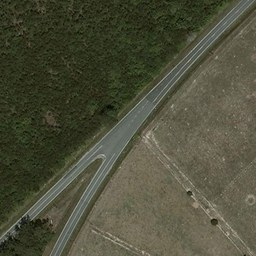
\includegraphics[height=2.1cm]{f1_aerial.jpg}};
    \node[lbl] at (1.05,-1.35) {aerial tile (input)};
    \node[frz, minimum width=2.2cm, minimum height=0.9cm, text width=2.0cm] (dino) at (3.6,1.05) {DINOv2-S/14\\(frozen)};
    \node[trn, minimum width=2.6cm, minimum height=0.9cm, text width=2.4cm] (pol) at (6.5,1.05) {\textbf{PolarLayoutNet}\\(trained)};
    \node[inner sep=0] (lay) at (9.2,1.05) {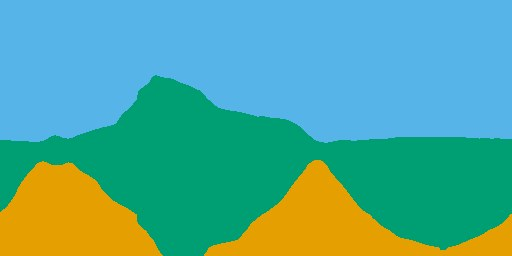
\includegraphics[width=2.2cm]{f1_layout.jpg}};
    \node[lbl] at (9.2,1.85) {predicted layout};
    \node[blk, minimum width=2.2cm, minimum height=0.9cm, text width=2.0cm] (warp) at (3.6,-1.05) {polar warp\\(fixed geometry)};
    \node[inner sep=0] (wim) at (9.2,-1.05) {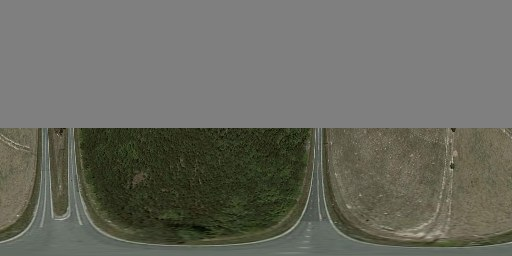
\includegraphics[width=2.2cm]{f1_warp.jpg}};
    \node[lbl] at (9.2,-1.85) {warped aerial};
    \node[trn, minimum width=1.5cm, minimum height=0.9cm, text width=1.3cm] (g) at (11.6,0) {\textbf{SPADE}\\generator};
    \node[inner sep=0] (gen) at (14.0,1.05) {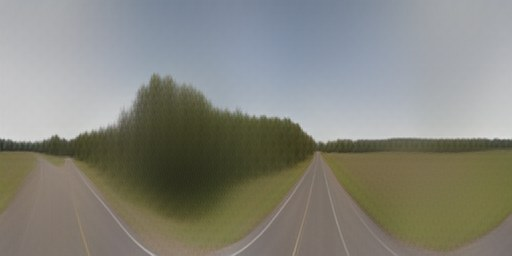
\includegraphics[width=2.2cm]{f1_gen.jpg}};
    \node[lbl] at (14.0,1.85) {generated (Config E)};
    \node[inner sep=0] (real) at (14.0,-1.05) {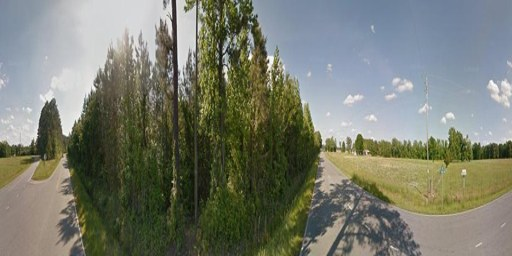
\includegraphics[width=2.2cm]{f1_real.jpg}};
    \node[lbl] at (14.0,-1.85) {real panorama (not an input)};
    \draw[arr] ($(aer.east)+(0,0.55)$) -- (dino.west);
    \draw[arr] ($(aer.east)+(0,-0.55)$) -- (warp.west);
    \draw[arr] (dino) -- (pol);
    \draw[arr] (pol) -- (lay);
    \draw[arr] (warp.east) -- (wim.west);
    \draw[arr] (lay.east) -- (g.north west);
    \draw[arr] (wim.east) -- (g.south west);
    \draw[arr] (g.east) -- (gen.west);
  \end{tikzpicture}
  \caption{Pipeline on test image 500 (Config E, LPIPS 0.624, the 43rd percentile of the test set). Blue:
  frozen; orange: trained. Stage~1 encodes the tile with a frozen DINOv2 backbone and a trained
  PolarLayoutNet; the polar warp has no learned parameters. The SPADE generator (Stage~2) receives the
  predicted layout and the warped tile's pixels; it is trained with oracle layouts and sees predicted layouts
  only at test time. Layout colours: \swatch{oiSkyBlue} sky/other, \swatch{oiGreen} vegetation,
  \swatch{oiOrange} road, \swatch{oiPurple} building.}
  \label{fig:teaser}
\end{figure}

% ==================================================================================================
\section{Related Work}
\label{sec:related}

\paragraph{Cross-view GANs and geometry.} Regmi and Borji \cite{regmi2018crossview} synthesise
aerial-to-street views with conditional GANs that also generate the target-view segmentation. SelectionGAN
\cite{tang2019selectiongan} conditions on an image and a target semantic map and refines a coarse result with
multi-channel attention selection. S2SP \cite{shi2022s2sp} establishes explicit geometric correspondences and
projects the satellite image to the street viewpoint before generation, and Toker et al.\ \cite{toker2021cdte}
train street-view synthesis jointly with cross-view retrieval. Our warped-aerial input is a much simpler,
fixed polar resampling in the same spirit.

\paragraph{Density- and diffusion-based methods.} Sat2Density \cite{qian2023sat2density} learns a density
field from satellite-ground pairs without depth supervision, and Sat2Density++ \cite{qian2025sat2density}
learns a neural radiance field to render street-view panoramas and videos. CrossViewDiff
\cite{li2024crossviewdiff} conditions a diffusion model on estimated satellite scene structure and
cross-view texture mapping, and its Table~1 collects the CVUSA numbers we quote in \cref{tab:published}.

\paragraph{Layout prediction.} CrossNet \cite{zhai2017crossnet} predicts the ground-level semantic layout from
aerial imagery, supervised by segmentations of co-located ground images, and uses aerial features to
hallucinate a plausible panorama. It is our Stage~1 baseline. CVUSA was introduced for cross-view
geolocalisation \cite{workman2015cvusa}.

\paragraph{Foundation features and semantic synthesis.} DINOv2 \cite{oquab2023dinov2} provides
all-purpose visual features that work without fine-tuning; register tokens \cite{darcet2023registers} remove
high-norm artefacts and give smoother feature maps. Pix2Pix \cite{isola2017pix2pix} learns image-to-image
mappings with a conditional adversarial loss. SPADE \cite{park2019spade} injects the semantic layout through
spatially-adaptive normalisation so that the layout is not washed out by normalisation layers. Our
contribution is not a new generator but a controlled measurement: we keep the encoder frozen, make the
predicted layout an explicit bottleneck, quantify its cost with oracle layouts, and report paired intervals
for every per-image comparison.

% ==================================================================================================
\section{Method}
\label{sec:method}

\subsection{Data, labels and protocol}
\label{sec:data}
We use CVUSA \cite{workman2015cvusa} with its standard split of \num{35532} training and \num{8884} test pairs.
Each pair holds a $750\times750$ aerial tile and a $1232\times224$ street-view panorama whose centre is the
tile centre. The released code calls the test split ``val''; we call it the test set throughout.

CVUSA provides no street-view semantic labels. We label every panorama with SegFormer-B0
\cite{xie2021segformer} fine-tuned on ADE20K and map its classes to four: sky, vegetation, road and building (the mapping is listed in
\cref{app:labelmap}). The four classes are coarse groups rather than pure categories: class~0 combines sky and
water with every ADE20K class we did not assign elsewhere (for example person, pole and signboard), so we call
it sky/other; class~1 groups vegetation with natural terrain such as mountain, rock, sand, hill and land;
class~2 includes vehicles and bare earth; and class~3 includes other built structures such as fences, railings
and bridges, which may partly explain its low IoU.
Relabelling \num{44416} pairs took 132.2 minutes. These pseudo-labels are the Stage~1 targets and the
Stage~2 oracle layouts, and all mIoU numbers use them. For Stage~1 model selection we hold
out a \num{2000}-image minival set from the training split (seed 0) and train on the remaining \num{33532}.

\subsection{Stage 1: PolarLayoutNet}
\label{sec:stage1}

\begin{figure}[t]
  \centering
  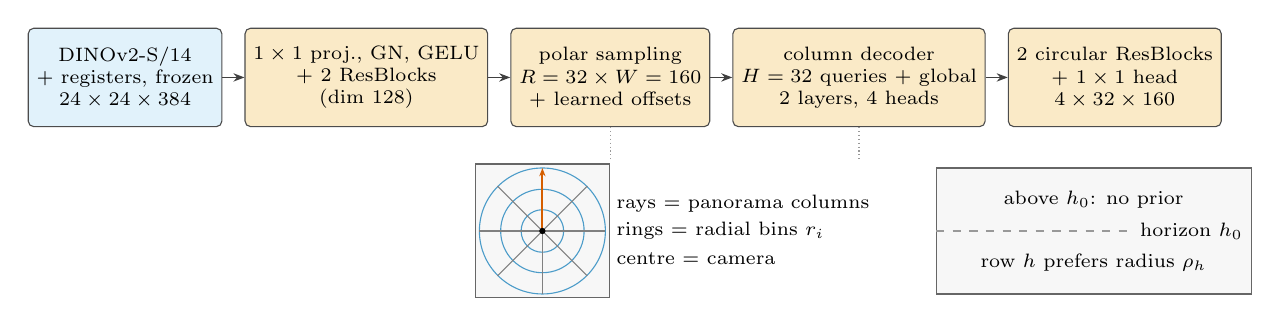
\begin{tikzpicture}[node distance=2.8mm, blk/.append style={font=\scriptsize}]
    \node[frz, minimum height=1.25cm] (in) {DINOv2-S/14\\+ registers, frozen\\$24\times24\times384$};
    \node[trn, right=of in, minimum height=1.25cm] (proj) {$1\times1$ proj., GN, GELU\\+ 2 ResBlocks\\(dim 128)};
    \node[trn, right=of proj, minimum height=1.25cm] (polar) {polar sampling\\$R=32\times W=160$\\+ learned offsets};
    \node[trn, right=of polar, minimum height=1.25cm] (dec) {column decoder\\$H=32$ queries + global\\2 layers, 4 heads};
    \node[trn, right=of dec, minimum height=1.25cm] (ref) {2 circular ResBlocks\\+ $1\times1$ head\\$4\times32\times160$};
    \draw[arr] (in) -- (proj);
    \draw[arr] (proj) -- (polar);
    \draw[arr] (polar) -- (dec);
    \draw[arr] (dec) -- (ref);
    % polar sampling inset
    \begin{scope}[shift={(5.3cm,-1.95cm)}]
      \draw[black!60, fill=black!3] (-0.85cm,-0.85cm) rectangle (0.85cm,0.85cm);
      \draw[oiBlue!70] (0,0) circle [radius=0.27cm];
      \draw[oiBlue!70] (0,0) circle [radius=0.53cm];
      \draw[oiBlue!70] (0,0) circle [radius=0.8cm];
      \draw[oiVermillion, line width=0.7pt, -{Stealth[length=3pt]}] (0,0) -- (0,0.8cm);
      \draw[black!50] (0,0) -- (0.57cm,0.57cm);
      \draw[black!50] (0,0) -- (0.8cm,0);
      \draw[black!50] (0,0) -- (0.57cm,-0.57cm);
      \draw[black!50] (0,0) -- (0,-0.8cm);
      \draw[black!50] (0,0) -- (-0.57cm,-0.57cm);
      \draw[black!50] (0,0) -- (-0.8cm,0);
      \draw[black!50] (0,0) -- (-0.57cm,0.57cm);
      \fill (0,0) circle [radius=0.04cm];
      \node[lbl, right] at (0.9cm,0.35cm) {rays $=$ panorama columns};
      \node[lbl, right] at (0.9cm,0) {rings $=$ radial bins $r_i$};
      \node[lbl, right] at (0.9cm,-0.35cm) {centre $=$ camera};
    \end{scope}
    \begin{scope}[shift={(12.3cm,-1.95cm)}]
      \draw[black!60, fill=black!3] (-2.0cm,-0.8cm) rectangle (2.0cm,0.8cm);
      \draw[black!40, dashed] (-2.0cm,0) -- (0.5cm,0);
      \node[lbl, right] at (0.55cm,0) {horizon $h_0$};
      \node[lbl] at (0,0.4cm) {above $h_0$: no prior};
      \node[lbl] at (0,-0.4cm) {row $h$ prefers radius $\rho_h$};
    \end{scope}
    \draw[black!40, densely dotted] (polar.south) -- ++(0,-0.4cm);
    \draw[black!40, densely dotted] (dec.south) -- ++(0,-0.4cm);
  \end{tikzpicture}
  \caption{PolarLayoutNet. Frozen DINOv2 tokens of the full tile are projected, resampled along rays from the
  tile centre (one ray per panorama column), decoded column by column with attention biased by a ground-plane
  prior, and refined with circular padding so that the panorama wraps around. Only the orange blocks are
  trained (1.53M parameters).}
  \label{fig:polarnet}
\end{figure}

\paragraph{Features.} The full $750\times750$ tile is resized to $336\times336$ and encoded once with
DINOv2-S/14 with registers \cite{oquab2023dinov2,darcet2023registers}; the $24\times24\times384$ patch grid is
cached in half precision. A $1\times1$ projection to 128 channels, GroupNorm, GELU and two residual blocks
produce the feature map $\mathbf{F}$ (\cref{fig:polarnet}).

\paragraph{Polar sampling.} Each panorama column corresponds to an azimuth and each ground pixel to a distance
from the camera. We therefore resample $\mathbf{F}$ on $R=32$ radial bins and $W=160$ azimuths,
\begin{equation}
  r_i=\frac{i+0.5}{R},\qquad \theta_j=\frac{2\pi(j+0.5)}{W}-\pi,\qquad
  \mathbf{p}_{ij}=\big(r_i\sin\theta_j,\;-r_i\cos\theta_j\big),
  \label{eq:polar}
\end{equation}
in normalised tile coordinates, with bilinear sampling $\mathbf{P}_{ij}=\mathbf{F}(\mathbf{p}_{ij}+0.1\tanh
\boldsymbol{\delta}_{ij})$. The offsets $\boldsymbol{\delta}$ come from a zero-initialised convolution over
the first sampling pass. A learned radial embedding is added to every sample.

\paragraph{Column decoder.} For every azimuth $j$, $H=32$ learned row queries attend over that column's $R$
samples plus one global token, a linear map of the mean of $\mathbf{F}$. The decoder has two pre-norm layers
with 4 heads and a feed-forward width of twice the model dimension, and is shared across columns. Its
attention logits receive an additive bias initialised from a ground-plane prior: with horizon row
$h_0=0.5H$, a row $h$ below the horizon prefers the radius $\rho_h$ at which the ground would appear,
\begin{equation}
  \rho_h=\min\!\Big(1,\frac{H-(h+0.5)}{H-h_0}\Big),\qquad
  b_{hi}=-\frac{1}{2}\Big(\frac{(r_i-\rho_h)R}{1.5}\Big)^{2},
  \label{eq:prior}
\end{equation}
and rows above the horizon receive $b_{hi}=0$. The bias stays trainable. Two residual blocks with circular padding along the
azimuth and a $1\times1$ head produce $4\times32\times160$ logits, which are bilinearly upsampled to
$224\times1232$ for evaluation.

\paragraph{Loss and training.} We minimise focal loss \cite{lin2017focal} plus soft Dice loss
(\cref{eq:s1loss} in \cref{app:hyper}) on labels at head resolution, train for 8 epochs with AdamW and keep the
checkpoint with the best minival mIoU.

\subsection{Stage 2: layout-to-panorama generators}
\label{sec:stage2}

\paragraph{Generators.} The Pix2Pix U-Net baseline \cite{isola2017pix2pix} (54.42M parameters) maps the
one-hot layout to RGB. It is warm-started from step \num{197766} (epoch 38) of an earlier run on a previous
label version (from our course project) and fine-tuned for 15 epochs with $\lambda_{L1}=100$ and no perceptual loss. The SPADE generator
\cite{park2019spade} (92.09M parameters) starts from the conditioning map downsampled to $8\times16$, applies
seven SPADE residual blocks with five $2\times$ nearest-neighbour upsamplings, and outputs $256\times512$ RGB;
every normalisation layer is modulated by the resized conditioning map (hidden width 128). There is no noise
input, so the generator is deterministic.

\paragraph{Warped-aerial conditioning.} We resample the aerial RGB tile into panorama geometry with a fixed
polar grid: the tile centre maps to the bottom row, the tile edge to the horizon row, azimuth runs clockwise,
and north sits at the centre column. The orientation was calibrated once on 400 training pairs by matching
warped and panorama road masks. Rows above the horizon are set to zero. The three warped channels are
concatenated with the four layout channels (layout resized with nearest neighbour, aerial bilinearly), which
adds 0.09M parameters (92.18M in total). \Cref{fig:app_warp} shows two warps.

\paragraph{Losses and discriminator.} A conditional PatchGAN discriminator $D$ (2.77M parameters) sees the
layout concatenated with a real or generated image; it receives the layout only, not the warped aerial. We use
least-squares GAN losses \cite{mao2017lsgan} with a smoothed real target of 0.9,
\begin{equation}
  \mathcal{L}_D=\tfrac{1}{2}\big[(D(x)-0.9)^2+D(\hat x)^2\big],\qquad
  \mathcal{L}_G=(D(\hat x)-1)^2+\lambda_{L1}\lVert\hat x-x\rVert_1
  +\lambda_{p}\sum_{l}\lVert\phi_l(\hat x)-\phi_l(x)\rVert_1,
  \label{eq:gan}
\end{equation}
where $\phi_l$ are the relu1\_1 to relu4\_1 activations of an ImageNet VGG-19 (4 layers) as a perceptual loss
\cite{johnson2016perceptual}. SPADE uses $\lambda_{L1}=\lambda_p=10$. All Stage~2 models train for 15 epochs
(\num{2220} steps per epoch) with batch 16, Adam ($\beta=(0.5,0.999)$, learning rate \num{2e-4}), 3 generator
steps
per discriminator step and mixed precision. $D$ is randomly initialised in every evaluated configuration
(A--E); a warm-started $D$ failed in our diagnostic runs (\cref{sec:diagnostics}). Generators are always
trained on oracle layouts.

\subsection{End-to-end inference}
\label{sec:inference}
At test time Stage~1 logits are bilinearly upsampled to $256\times512$, converted by argmax to a one-hot layout
in $[-1,1]$, and passed to the generator together with the warped aerial image. Stage~2 never sees a predicted
layout in training, so Configs C and E also measure this train-test shift.

% ==================================================================================================
\section{Experimental Setup}
\label{sec:setup}

\paragraph{Metrics.} Stage~1 reports pixel accuracy, per-class IoU and mIoU over all \num{8884} test panoramas
at $224\times1232$. For Stage~2 we compute, per test image at $256\times512$, SSIM, PSNR, LPIPS with AlexNet
features \cite{zhang2018lpips} and a \emph{Laplacian sharpness gap}
$\lvert\operatorname{Var}(\nabla^2 Y)-\operatorname{Var}(\nabla^2\hat Y)\rvert$ on 8-bit luma $Y$. This gap
is our own measure and is not the SD metric of prior work. Set-level clean-FID \cite{parmar2022cleanfid,
heusel2017fid} and KID \cite{binkowski2018kid} use all \num{8884} generated and real panoramas. An older
torchvision-Inception harness, which we call \emph{legacy FID}, appears only in \cref{app:legacy}. Per-image
SSIM uses scikit-image \texttt{structural\_similarity} on uint8 RGB after mapping generator outputs from
$[-1,1]$ to eight-bit RGB, with \texttt{channel\_axis=2}, \texttt{data\_range=255}, default
\texttt{win\_size=7} and uniform filter weights (\texttt{gaussian\_weights=False}). PSNR uses scikit-image
\texttt{peak\_signal\_noise\_ratio} on the same uint8 RGB tensors with \texttt{data\_range=255}. LPIPS uses
the \texttt{lpips} package with AlexNet (\texttt{net='alex'}), leaving inputs in $[-1,1]$. clean-FID and KID
call \texttt{cleanfid} with \texttt{mode='clean'} and batch size 32 on folders of $256\times512$ PNG RGB images
written by \texttt{final\_eval.py}; clean-FID applies its own resizing and normalisation internally
\cite{parmar2022cleanfid}.

\paragraph{Uncertainty.} Each model was trained once, so our intervals capture test-set sampling, not
training variance. Per-image metrics get 95\% percentile intervals from \num{1000} bootstrap resamples of test
images (seed 0); for D vs B and E vs C we bootstrap the per-image paired differences. FID and KID have no
intervals. We call a difference significant only when its 95\% interval excludes zero. Differences quoted in
the text are computed from unrounded values, so they can differ by up to 0.001 (0.1 for FID) from differences
of the rounded table entries.

\begin{table}[t]
  \centering
  \small
  \caption{Stage~2 configurations. The oracle layout is the SegFormer segmentation of the target panorama; the
  predicted layout is the Stage~1 output. Each uses the last checkpoint saved by its training run.}
  \label{tab:configs}
  \begin{tabular}{c l l c r}
    \toprule
    Config & Generator & Layout at test time & Warped aerial & Generator step \\
    \midrule
    A & Pix2Pix U-Net (54.42M) & oracle & -- & \num{231066} \\
    B & SPADE (92.09M) & oracle & -- & \num{33300} \\
    C & SPADE (92.09M) & predicted & -- & \num{33300} \\
    D & SPADE + aerial (92.18M) & oracle & \checkmark & \num{32000} \\
    E & SPADE + aerial (92.18M) & predicted & \checkmark & \num{32000} \\
    \bottomrule
  \end{tabular}
\end{table}

\paragraph{Configurations.} In \cref{tab:configs}, B and C share one checkpoint, as do D and E, so C$-$B
and E$-$D isolate the layout source. D$-$B and E$-$C isolate warped-aerial conditioning up to the training-run
differences noted in \cref{sec:ladder}. Stage~2 had no separate validation split. Several checkpoints of the
same runs were scored on the test split during development (\cref{app:legacy}), and the Pix2Pix, SPADE and
aerial configurations were compared on the same test images while they were being developed, so test data may
have influenced which runs and settings we kept; each configuration reports the last checkpoint its run saved.

\paragraph{Compute.} Summed over the logs, Stage~1 used 27.6 GPU-hours, Stage~2 16.3 and the final
evaluation 1.70, 45.6 GPU-hours in total; relabelling adds 2.20. \Cref{app:compute} gives the per-run
breakdown, the GPUs named in the logs and what was not recorded.

% ==================================================================================================
\section{Results}
\label{sec:results}

\subsection{Stage 1 layout prediction}
\label{sec:s1main}

\begin{table}[t]
  \centering
  \small
  \caption{Stage~1 on the CVUSA test set (\num{8884} panoramas), scored against SegFormer pseudo-labels. The
  original CrossNet checkpoint was trained on its own labels, so its gap mixes label and architecture effects;
  the retrained CrossNet isolates the architecture. Best per column in bold. ``Sky'' denotes the sky/other class
  (\cref{app:labelmap}).}
  \label{tab:stage1}
  \setlength{\tabcolsep}{5pt}
  \begin{tabular}{l c cc cccc}
    \toprule
    Method & Trained on & mIoU$\uparrow$ & Acc.$\uparrow$ & Sky & Veg. & Road & Bldg. \\
    \midrule
    CrossNet \cite{zhai2017crossnet}, original checkpoint & original labels & 0.299 & 0.434 & 0.638 & 0.026 & 0.438 & 0.095 \\
    CrossNet, retrained & our pseudo-labels & 0.402 & 0.665 & 0.633 & 0.533 & 0.362 & 0.080 \\
    PolarLayoutNet (ours) & our pseudo-labels & \textbf{0.514} & \textbf{0.745} & \textbf{0.689} & \textbf{0.661} & \textbf{0.494} & \textbf{0.209} \\
    \bottomrule
  \end{tabular}
\end{table}

PolarLayoutNet reaches 0.514 mIoU and 0.745 pixel accuracy (\cref{tab:stage1}). Against CrossNet retrained on
the same pseudo-labels, the gain is $+0.112$ mIoU, with every class improving (road $+0.132$, building
$+0.129$, vegetation $+0.129$, sky $+0.056$). Against the original CrossNet checkpoint the gain is $+0.214$,
but that checkpoint never saw our label definition (it scores 0.454 on its own labels), so this larger number
should not be read as an architecture effect. The retrained baseline is, if anything, favoured: its checkpoint
was selected on a \num{1024}-image subset of the test split.

\Cref{fig:stage1} shows the first three test images. The original CrossNet predicts building where the
labels have vegetation, matching its vegetation IoU of 0.026, and the retrained CrossNet produces flat,
nearly horizontal class boundaries. Our predictions follow the road shape and the vegetation skyline more closely but still miss small
buildings, which is consistent with a building IoU of 0.209.

\begin{figure}[t]
  \centering
  \setlength{\imgw}{0.74\linewidth}
  \setlength{\tabcolsep}{2pt}
  \renewcommand{\arraystretch}{0.9}
  \begin{tabular}{@{}r l@{}}
    \rowlab{aerial} & \rowimg{f3_aerial.jpg} \\
    \rowlab{real panorama} & \rowimg{f3_real.jpg} \\
    \rowlab{pseudo-label} & \rowimg{f3_gt.jpg} \\
    \rowlab{CrossNet (orig.)} & \rowimg{f3_crossnet.jpg} \\
    \rowlab{CrossNet (retr.)} & \rowimg{f3_phase1.jpg} \\
    \rowlab{ours} & \rowimg{f3_ours.jpg} \\
  \end{tabular}
  \caption{Stage~1 predictions for test images 0, 1 and 2 (the first three test indices; no selection). The
  CrossNet panels are the predicted-layout panels from each model's evaluation output, recoloured to our
  palette. Colours as in \cref{fig:teaser}.}
  \label{fig:stage1}
\end{figure}

\noindent\textbf{Takeaway.} A small head on frozen DINOv2 features exceeds a retrained CrossNet by $+0.112$
mIoU on identical labels, at a training cost of about four GPU-hours.

\subsection{What matters in Stage 1}
\label{sec:s1abl}

\begin{table}[t]
  \centering
  \small
  \caption{Stage~1 single-change ablations on the test set. $\Delta$ is the mIoU change from the reference; each
  row is one run with one seed, so differences of a few thousandths are within run-to-run variation that we did
  not measure. VGG-16 gives a $21\times21$ grid and the crop a $16\times16$ grid; ``no prior'' starts the
  bias at zero and ``fixed prior'' freezes it. Bold marks the best value per column (ties at the displayed
  precision are all bold).
  $^{\ast}$Also uses mixed precision, batch 32 and a different GPU. $^{\dagger}$Also uses mixed precision.
  ``Sky'' denotes the sky/other class (\cref{app:labelmap}).}
  \label{tab:ablations}
  \setlength{\tabcolsep}{4.5pt}
  \begin{tabular}{@{}l c c r cccc@{}}
    \toprule
    Variant & Params (M) & mIoU$\uparrow$ & $\Delta$ & Sky & Veg. & Road & Bldg. \\
    \midrule
    Reference (\cref{sec:stage1}) & 1.53 & \textbf{0.514} & -- & 0.689 & 0.661 & 0.494 & 0.209 \\
    \addlinespace
    \multicolumn{8}{@{}l}{\emph{Input features}} \\
    \quad VGG-16 conv5 instead of DINOv2 & 1.55 & 0.485 & $-0.0283$ & 0.664 & 0.627 & 0.468 & 0.181 \\
    \quad $224$\,px centre crop instead of full tile & 1.53 & 0.502 & $-0.0117$ & 0.675 & 0.643 & 0.491 & 0.198 \\
    \addlinespace
    \multicolumn{8}{@{}l}{\emph{Cross-view mapping and decoder}} \\
    \quad dense mapping instead of polar & 4.48 & \textbf{0.514} & $+0.0002$ & 0.688 & 0.660 & \textbf{0.499} & 0.207 \\
    \quad no ground-plane prior & 1.53 & \textbf{0.514} & $+0.0004$ & 0.690 & 0.662 & 0.494 & 0.209 \\
    \quad fixed prior & 1.53 & 0.513 & $-0.0002$ & 0.688 & 0.660 & 0.495 & 0.210 \\
    \quad no learned offsets & 1.53 & \textbf{0.514} & $+0.0007$ & \textbf{0.691} & \textbf{0.663} & 0.497 & 0.206 \\
    \addlinespace
    \multicolumn{8}{@{}l}{\emph{Head and loss}} \\
    \quad $64\times320$ head$^{\ast}$ & 1.55 & 0.513 & $-0.0009$ & 0.684 & 0.657 & 0.496 & 0.214 \\
    \quad inverse-frequency weights$^{\dagger}$ & 1.53 & 0.501 & $-0.0129$ & 0.649 & 0.623 & 0.493 & \textbf{0.237} \\
    \bottomrule
  \end{tabular}
\end{table}

\Cref{tab:ablations} changes one factor at a time. Two changes matter. Replacing DINOv2 with frozen VGG-16
features costs 0.028 mIoU at a similar parameter count, and encoding a $224$\,px centre crop instead of the
full tile costs 0.012. The crop also coarsens the token grid, so the second effect combines coverage and
resolution.

The remaining changes form a null set. Dense mapping (a learned token-to-cell matrix with 2.9 times the
parameters), the three prior settings, the offsets and a finer $64\times320$ head all land within 0.001 mIoU of
the reference. Inverse-frequency class weights trade 0.013 mIoU for $+0.028$ building IoU.

\noindent\textbf{Takeaway.} In this setting the backbone and the input coverage matter, while the geometric
details of the decoder show no measurable effect in single runs; the decoder appears able to learn the
cross-view mapping without a hand-built prior.

\subsection{Stage 2: the configuration ladder}
\label{sec:ladder}

\begin{table}[t]
  \centering
  \small
  \caption{Stage~2 results on the test set ($256\times512$, \num{8884} images). Grey brackets: 95\% bootstrap
  intervals over test images (none for set-level FID and KID). Sharp.\ gap: our Laplacian sharpness gap. Bold
  marks the best point estimate per block, not significance (E vs C SSIM is not significant, \cref{tab:paired}).}
  \label{tab:ladder}
  \setlength{\tabcolsep}{4pt}
  \begin{tabular}{c l cccc cc}
    \toprule
    Config & Generator & SSIM$\uparrow$ & PSNR$\uparrow$ & LPIPS$\downarrow$ & Sharp.\ gap$\downarrow$ & clean-FID$\downarrow$ & KID$\downarrow$ \\
    \midrule
    \multicolumn{8}{@{}l}{\emph{Oracle layout}} \\
    A & Pix2Pix U-Net & \textbf{0.516} & 17.07 & 0.610 & 622 & 167.4 & 0.180 \\[-2pt]
      & & \ci{0.513}{0.518} & \ci{17.02}{17.13} & \ci{0.608}{0.612} & \ci{614}{630} & & \\
    B & SPADE & 0.507 & 17.06 & 0.591 & 592 & 155.4 & 0.179 \\[-2pt]
      & & \ci{0.504}{0.509} & \ci{17.01}{17.11} & \ci{0.588}{0.594} & \ci{584}{600} & & \\
    D & SPADE + aerial & 0.509 & \textbf{17.28} & \textbf{0.565} & \textbf{586} & \textbf{141.0} & \textbf{0.163} \\[-2pt]
      & & \ci{0.506}{0.511} & \ci{17.23}{17.33} & \ci{0.562}{0.567} & \ci{578}{594} & & \\
    \midrule
    \multicolumn{8}{@{}l}{\emph{Predicted layout (end-to-end)}} \\
    C & SPADE & 0.458 & 14.65 & 0.671 & 597 & 195.0 & 0.221 \\[-2pt]
      & & \ci{0.456}{0.461} & \ci{14.60}{14.69} & \ci{0.668}{0.673} & \ci{588}{604} & & \\
    E & SPADE + aerial & \textbf{0.459} & \textbf{14.82} & \textbf{0.650} & \textbf{592} & \textbf{182.1} & \textbf{0.209} \\[-2pt]
      & & \ci{0.456}{0.461} & \ci{14.78}{14.87} & \ci{0.647}{0.652} & \ci{584}{600} & & \\
    \bottomrule
  \end{tabular}
\end{table}

\begin{table}[t]
  \centering
  \small
  \caption{Paired differences for warped-aerial conditioning (with minus without), with 95\% bootstrap
  intervals over per-image differences. The last column is the share of test images whose LPIPS improves. FID
  and KID differences are set-level and have no intervals. The two runs also differ in learning-rate schedule
  and resume history (\cref{sec:ladder}).}
  \label{tab:paired}
  \setlength{\tabcolsep}{4pt}
  \begin{tabular}{l ccc cc c}
    \toprule
    Comparison & $\Delta$SSIM & $\Delta$PSNR (dB) & $\Delta$LPIPS & $\Delta$clean-FID & $\Delta$KID & LPIPS lower \\
    \midrule
    D$-$B (oracle) & $+0.00196$ & $+0.23$ & $-0.026$ & $-14.3$ & $-0.016$ & 87.0\% \\[-2pt]
      & \ci{+0.00168}{+0.00223} & \ci{+0.20}{+0.25} & \ci{-0.027}{-0.026} & & & \\
    E$-$C (predicted) & $+0.00019$ & $+0.17$ & $-0.021$ & $-12.9$ & $-0.012$ & 85.3\% \\[-2pt]
      & \ci{-0.00003}{+0.00043} & \ci{+0.16}{+0.19} & \ci{-0.021}{-0.020} & & & \\
    \bottomrule
  \end{tabular}
\end{table}

\Cref{tab:ladder} and \cref{fig:ladder} give the full ladder. With oracle layouts, SPADE (B) improves on the
Pix2Pix U-Net (A) by 0.019 LPIPS and 12.0 clean-FID, while A keeps a 0.009 higher SSIM. The two generators
differ in architecture, size, $\lambda_{L1}$, perceptual loss, learning-rate schedule and initialisation (A
was warm-started), so we read this only as evidence that SPADE is a reasonable base.

Adding the warped aerial image is the cleaner comparison (\cref{tab:paired}). With oracle layouts (D$-$B), LPIPS
falls by 0.026 and PSNR rises by 0.23\,dB, both intervals excluding zero, and 87.0\% of test images improve in
LPIPS. With predicted layouts (E$-$C), LPIPS falls by 0.021 and PSNR rises by 0.17\,dB, again excluding zero,
and 85.3\% of images improve; the SSIM change is not significant. Clean-FID point estimates fall by 14.3 (oracle) and 12.9 (predicted). One confound remains: the layout-only SPADE run decayed its learning rate linearly to zero after epoch 8, whereas the aerial run stayed at \num{2e-4} in every logged epoch and was resumed from step \num{12000}. The aerial run therefore lacked the annealing of the layout-only run, which would if anything disadvantage it; the resume history is a second difference we did not isolate.

\begin{figure}[t]
  \centering
  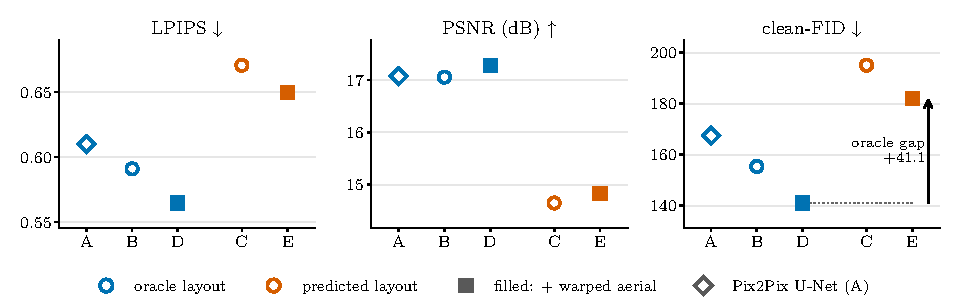
\includegraphics[width=0.92\linewidth]{f5_ladder.pdf}
  \caption{Stage~2 ladder. Points are test-set means; whiskers are 95\% bootstrap intervals (often smaller
  than the marker); clean-FID has no interval. Blue: oracle layout; vermillion: predicted layout; filled
  squares: with warped aerial. The arrow marks the oracle gap between D and E.}
  \label{fig:ladder}
\end{figure}

\noindent\textbf{Takeaway.} Warped-aerial conditioning gives a small, consistent LPIPS improvement with both
layout sources and lowers clean-FID by 14.3 and 12.9, although the two runs also differ in schedule.

\subsection{The oracle gap}
\label{sec:gap}

The largest effect in the study is the layout source. Moving from oracle to predicted layouts with the same
checkpoint raises clean-FID by 41.1 (D to E: 141.0 to 182.1), LPIPS by 0.085 and KID by 0.047, and lowers PSNR
by 2.46\,dB and SSIM by 0.050. Without the aerial input the gap is similar (39.6 clean-FID, B to C). In clean-FID
the oracle gap is 2.9 times the warped-aerial gain, and in LPIPS it is 3.2 times. Part of the gap may come from
the train-test shift in \cref{sec:inference}, because the generator never saw predicted layouts during
training; the two causes are not separated here.

\noindent\textbf{Takeaway.} The largest effect we measure is the layout source: a perfect layout would be
worth roughly three times what the aerial image adds, although we cannot separate Stage~1 error from the
train--test mismatch.

\subsection{Qualitative results and failure cases}
\label{sec:qual}

\begin{figure}[t]
  \centering
  \setlength{\imgw}{0.64\linewidth}
  \setlength{\tabcolsep}{2pt}
  \renewcommand{\arraystretch}{0.9}
  \begin{tabular}{@{}r l@{}}
    & \collabel{best (8870)}\collabel{25th pct.\ (4277)}\collabel{median (5554)}\collabel{75th pct.\ (6128)}\collabel{worst (654)} \\
    \rowlab{aerial} & \rowimg{f4_aerial.jpg} \\
    \rowlab{pred.\ layout} & \rowimg{f4_pred.jpg} \\
    \rowlab{oracle layout} & \rowimg{f4_gt.jpg} \\
    \rowlab{A} & \rowimg{f4_A.jpg} \\
    \rowlab{B} & \rowimg{f4_B.jpg} \\
    \rowlab{D} & \rowimg{f4_D.jpg} \\
    \rowlab{E} & \rowimg{f4_E.jpg} \\
    \rowlab{real} & \rowimg{f4_real.jpg} \\
  \end{tabular}
  \caption{End-to-end grid. Columns are the test images at the best, 25th percentile, median, 75th percentile
  and worst Config E LPIPS (0.295, 0.569, 0.645, 0.733 and 1.024); test indices in brackets. All panels were
  regenerated from the released checkpoints with the evaluation code, and their LPIPS matches the stored
  per-image values. Colours as in \cref{fig:teaser}.}
  \label{fig:grid}
\end{figure}

\Cref{fig:grid} samples Config E by its own LPIPS quantiles. On open roads (best and 25th percentile) the
predicted layout recovers the road shape and the generator produces a plausible, blurry scene. At the median
and 75th percentile, the predicted vegetation skyline differs from the oracle and the outputs inherit that
error; D shares E's weights but receives the oracle layout. The worst case is a forest view in
which both layouts are almost entirely vegetation and every generator returns a uniform blur;
Figure~\ref{fig:app_fail} shows six uncurated samples; the next three worst cases (test images 2955, 668 and
35) are also dense vegetation scenes with a nearly uniform predicted layout (LPIPS 1.012, 1.010 and 1.001).
All samples are far blurrier than the real panoramas.

\noindent\textbf{Takeaway.} Visible errors track layout errors, and the low-texture outputs explain why
pixel metrics look acceptable while clean-FID stays high.

% ==================================================================================================
\section{Training Diagnostics}
\label{sec:diagnostics}

\begin{figure}[t]
  \centering
  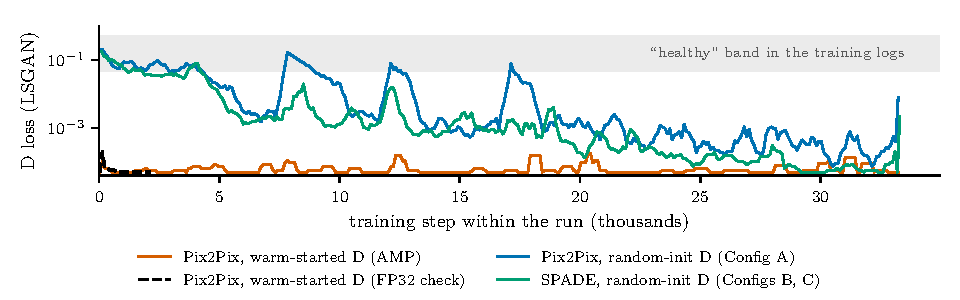
\includegraphics[width=0.9\linewidth]{f6_dloss.pdf}
  \caption{Discriminator loss logged every 100 steps, smoothed with a five-point geometric moving average
  (log scale). Logged values of 0.0000 are drawn at the floor of \num{5e-5}. The grey band is the ``healthy''
  range printed by the training script. The warm-started runs sit at the floor from step one; random
  initialisation starts inside the band but leaves it within the first few thousand steps.}
  \label{fig:dloss}
\end{figure}

Our first Pix2Pix fine-tuning warm-started both generator and discriminator from the earlier run, and its
discriminator was saturated from the first step (\cref{fig:dloss}). An instrumented FP32 run (warm-started
weights, a fresh optimiser state and one generator step per discriminator step) shows the mechanism: at step
one the discriminator output was 0.899 on real images, almost exactly the
smoothed target of 0.9, and 0.000 on generated images. Over 20 diagnostic lines up to step 500 the real mean
stayed between 0.876 and 0.910, the fake output never exceeded 0.009 in magnitude, and every logged
discriminator loss was below 0.05, the lower edge of the script's healthy band. The mixed-precision run
behaved the same way, which rules out mixed-precision underflow as the cause.

A third diagnostic run in FP32 changed two things at once, a randomly initialised discriminator and three
generator steps per discriminator step, and behaved as hoped: at step one both outputs were close to zero
($-0.085$ real, $-0.083$ fake), the epoch-average discriminator loss was 0.0966 and 0.1032 in its two
epochs, and only 20\% of logged steps fell below 0.05. Because the two changes were made together, we cannot
attribute the improvement to initialisation alone.

The full runs with random initialisation started in this range but did not stay there. For Config A (Pix2Pix)
the share of logged steps with discriminator loss below 0.05 rose from 27\% in the first epoch to 92\% from the
third epoch on, and the epoch-average loss fell from 0.1220 to 0.0009. For SPADE (Configs B and C) the share
rose from 50\% to 99\% and the average fell from 0.0879 to 0.0001; in the last epoch the adversarial loss
averaged 1.00, against weighted L1 and perceptual terms (after multiplying by their weights of 10) of 1.20 and
18.6. The aerial run, logged from epoch 6, was
below 0.05 at 99\% of logged steps. We read this as a discriminator with little useful gradient left: the
adversarial term was largely inactive after the first epochs.

\noindent\textbf{Takeaway.} A warm-started discriminator can saturate before training starts. Random
initialisation (together with three generator steps per discriminator step) restores the early dynamics but
not the late collapse, so the reported generators should be read as mostly reconstruction-trained.

% ==================================================================================================
\section{Discussion and Limitations}
\label{sec:discussion}

\begin{table}[t]
  \centering
  \small
  \caption{Published CVUSA numbers, copied from Table~1 of CrossViewDiff \cite{li2024crossviewdiff} and checked
  against its PDF. \textbf{They are not comparable with ours}: resolution, protocol, FID implementation and
  labels differ, and we re-ran no published method. The published SD column is omitted (a different measure).}
  \label{tab:published}
  \begin{tabular}{l cccc}
    \toprule
    Method & SSIM$\uparrow$ & PSNR$\uparrow$ & FID$\downarrow$ & KID$\downarrow$ \\
    \midrule
    CDTE \cite{toker2021cdte} & 0.283 & 13.82 & 28.35 & 0.028 \\
    S2SP \cite{shi2022s2sp} & 0.319 & 13.69 & 27.31 & 0.021 \\
    Sat2Density \cite{qian2023sat2density} & 0.339 & 14.23 & 41.43 & 0.036 \\
    CrossViewDiff \cite{li2024crossviewdiff} & 0.371 & 12.00 & 23.67 & 0.018 \\
    \midrule
    \multicolumn{5}{@{}l}{\emph{This study, our protocol (clean-FID)}} \\
    Config D (oracle layout) & 0.509 & 17.28 & 141.0 & 0.163 \\
    Config E (end-to-end) & 0.459 & 14.82 & 182.1 & 0.209 \\
    \bottomrule
  \end{tabular}
\end{table}

\paragraph{Where the pipeline stands.} Our end-to-end clean-FID of 182.1 is far behind the published FID range
of 24--41 (\cref{tab:published}), even allowing for protocol differences. Our higher SSIM and PSNR do not
indicate better synthesis: these metrics reward smooth outputs, and our samples are visibly blurrier
(\cref{fig:grid}).

\paragraph{Limitations.} All labels are SegFormer pseudo-labels, so mIoU measures agreement with another model
rather than with human annotation, and building IoU is only 0.21; there is no human evaluation of the
synthesised panoramas. We use one dataset, CVUSA, which covers the United States, and make no claim about
other datasets or regions. The $1232\times224$ panoramas are resized to $256\times512$ (height $\times$ width),
which changes their aspect ratio. Each configuration was trained once, so our intervals cover test-image
sampling only. The A-to-B and warped-aerial comparisons carry the confounds stated in \cref{sec:ladder}, the
adversarial term was largely inactive after the first epochs, and Stage~2 was trained only on oracle layouts.
We also did not train a generator conditioned on the warped aerial tile alone, so we cannot say whether the
layout stage helps relative to direct synthesis.

\paragraph{Future work.} The oracle gap points first to a better Stage~1 and to training Stage~2 on predicted
layouts, which would also separate layout error from train--test mismatch. A generator conditioned only on the
warped aerial tile would test whether the layout stage helps at all. A diffusion refiner with
ControlNet-style layout conditioning \cite{zhang2023controlnet} could add the missing texture, and a second
dataset and several training seeds would test how far the findings generalise.

% ==================================================================================================
\FloatBarrier
\section{Conclusion}
\label{sec:conclusion}

A 1.53M-parameter layout head on frozen DINOv2 features reaches 0.514 mIoU on CVUSA pseudo-labels, $+0.112$ over
a retrained CrossNet; the backbone and input coverage matter, the polar mapping details do not. A warped
aerial image lowers LPIPS with both layout sources, but the step from oracle to predicted layouts costs 41.1
clean-FID, the largest gap we measure, which points to Stage~1 quality, train--test mismatch, or both as the
first things to improve in this design. The released code, logs and checkpoints give a cheap, fully measured
baseline against which better layout prediction can be tested.
\label{endofmain}

\section*{Reproducibility and Data Statement}
Code, configuration files, training logs, the Stage~1 and Stage~2 checkpoints and the evaluation harness are
released at \url{https://github.com/anasahmed81103/AerialToGround} (release v1.0.0) \todo{confirm the release
and the Zenodo DOI are public before submission}. Every number in this paper was checked against the run
artefacts by a script shipped with the paper source (\texttt{paper/tools.py}). CVUSA was obtained from the
authors' shared Dropbox folder (\texttt{cvusa\_sharing}), following a data-access request to Nathan Jacobs
(Washington University in St. Louis), is used for research under its terms, and is not redistributed by us; the
figures show \num{17} distinct test images, identified in their captions.

\section*{Author Contributions}
A.A. and H.V. jointly developed the original CrossNet and Pix2Pix baselines in a shared course project. A.A.
designed and implemented Stages~1 and~2, ran all experiments and analyses, and wrote the paper \todo{confirm
contributions with H.V.}.

\section*{Acknowledgements}
This work began as a Computer Vision course project at FAST-NUCES; the original CrossNet checkpoint and the
Pix2Pix initialisation of Config A come from that project. This research received no external funding; cloud
GPU time was paid for personally by the first author. AI assistants (Cursor and Claude)
were used to help write analysis code and to draft and edit the text; the authors checked all results and
claims against the run artefacts and take responsibility for the content \todo{confirm venue policy}.

% ==================================================================================================
\appendix

\section{Hyperparameters}
\label{app:hyper}

With softmax probabilities $q$ and one-hot targets $y$ over $N$ pixels and $C$ classes, the Stage~1 loss is
\begin{equation}
  \mathcal{L}_{\mathrm{seg}}=-\frac{1}{N}\sum_{n}(1-q_{n,y_n})^{\gamma}\log q_{n,y_n}
  +\frac{1}{C}\sum_{c}\Big(1-\frac{2\sum_n q_{nc}y_{nc}+1}{\sum_n q_{nc}+\sum_n y_{nc}+1}\Big),
  \qquad \gamma=2,
  \label{eq:s1loss}
\end{equation}
computed on labels downsampled to the $32\times160$ head resolution. Training uses horizontal flips of tile and
panorama and the settings in \cref{tab:hyper}.

\begin{table}[h]
  \centering
  \small
  \caption{Training hyperparameters, read from the run configurations and logs.}
  \label{tab:hyper}
  \setlength{\tabcolsep}{4pt}
  \begin{tabular}{@{}>{\raggedright\arraybackslash}p{3.0cm} >{\raggedright\arraybackslash}p{5.5cm} >{\raggedright\arraybackslash}p{7.3cm}@{}}
    \toprule
    & Stage~1 (PolarLayoutNet) & Stage~2 (SPADE; Pix2Pix where different) \\
    \midrule
    Input & DINOv2-S/14 tokens, $24\times24\times384$ & one-hot layout (+ warped aerial), $256\times512$ \\
    Output & $4\times32\times160$ logits & $3\times256\times512$ RGB \\
    Trainable parameters & 1.53M & 92.09M / 92.18M (Pix2Pix 54.42M); $D$ 2.77M \\
    Optimiser & AdamW, lr \num{3e-4}, weight decay 0.01 & Adam, lr \num{2e-4}, $\beta=(0.5,0.999)$ \\
    Schedule & 500 warm-up steps, cosine & Layout SPADE: \num{2e-4} epochs 1--8, linear decay to 0 by epoch 15 (\num{33300} steps). SPADE + aerial: constant \num{2e-4} in logged epochs 6--15, resumed at step \num{12000}; checkpoint at \num{32000}. \\
    Batch, epochs & 16, 8 & 16, 15 (\num{2220} steps per epoch) \\
    Loss & focal ($\gamma=2$) + Dice & LSGAN + $10\,$L1 + $10\,$VGG-19 (Pix2Pix: $100\,$L1) \\
    Other & grad.\ clip 1.0, flip augmentation & real label 0.9, 3 $G$ steps per $D$ step, mixed precision \\
    Selection & best minival mIoU (\num{2000} train images) & last saved checkpoint \\
    \bottomrule
  \end{tabular}
\end{table}

\section{ADE20K to four-class label map}
\label{app:labelmap}

Relabelling follows \texttt{scripts/relabel\_cvusa.py}: SegFormer-B0 predicts ADE20K indices 0--149, which are
remapped to CrossNet-style ids 0 sky/other, 1 vegetation, 2 road and 3 building. Any ADE20K index not listed
below maps to sky/other (0).

\begin{table}[h]
  \centering
  \small
  \caption{ADE20K $\rightarrow$ four-class mapping (same as \texttt{\_ADE\_TO4} in \texttt{relabel\_cvusa.py}).}
  \label{tab:labelmap}
  \setlength{\tabcolsep}{3pt}
  \begin{tabular}{@{}c l p{9.2cm}@{}}
    \toprule
    Target & ADE20K id & ADE20K class name (\texttt{id2label} of \texttt{nvidia/segformer-b0-finetuned-ade-512-512}) \\
    \midrule
    \multirow{7}{*}{sky/other (0)} & 2 & sky \\
    & 21 & water \\
    & 26 & sea \\
    & 60 & river \\
    & 113 & waterfall \\
    & 128 & lake \\
    & \multicolumn{2}{@{}l@{}}{All other ADE20K indices (default in script)} \\
    \midrule
    \multirow{11}{*}{vegetation (1)} & 4 & tree \\
    & 9 & grass \\
    & 16 & mountain \\
    & 17 & plant \\
    & 29 & field \\
    & 34 & rock \\
    & 46 & sand \\
    & 66 & flower \\
    & 68 & hill \\
    & 72 & palm \\
    & 94 & land \\
    \midrule
    \multirow{10}{*}{road (2)} & 6 & road \\
    & 11 & sidewalk \\
    & 13 & earth \\
    & 20 & car \\
    & 52 & path \\
    & 54 & runway \\
    & 80 & bus \\
    & 83 & truck \\
    & 91 & dirt track \\
    & 102 & van \\
    \midrule
    \multirow{13}{*}{building (3)} & 0 & wall \\
    & 1 & building \\
    & 8 & windowpane \\
    & 14 & door \\
    & 25 & house \\
    & 32 & fence \\
    & 38 & railing \\
    & 42 & column \\
    & 48 & skyscraper \\
    & 61 & bridge \\
    & 79 & hovel \\
    & 84 & tower \\
    & 86 & awning \\
    \bottomrule
  \end{tabular}
\end{table}

\section{Compute}
\label{app:compute}

Stage~1 trains on the cached features; the main run took 234.1 minutes on a Quadro P1000 with 4\,GB of memory
and peaked at 1.98\,GB. Stage~2 runs used an RTX 4090 or an RTX PRO 4500 Blackwell, as stated in each log. The
full evaluation session, including clean-FID, KID and bootstrap, took about 6 hours (author-reported, not
logged).

\begin{table}[h]
  \centering
  \small
  \caption{GPU-hours as logged. Stage~1 times come from each run's results file and Stage~2 times from the sum
  of logged epoch times. GPU names come from the logs, except the rows marked local, the class-weighted row and
  the final-evaluation row, which are author-reported.}
  \label{tab:compute}
  \setlength{\tabcolsep}{4pt}
  \begin{tabular}{@{}l l r@{}}
    \toprule
    Run & GPU & GPU-hours \\
    \midrule
    Stage~1 reference (polar, full tile) & Quadro P1000 (4\,GB) & 3.90 \\
    Stage~1 ablations: no prior / fixed prior / no offsets & Quadro P1000 (local) & 3.91 / 3.87 / 3.70 \\
    Stage~1 ablations: dense / crop / VGG-16 & Quadro P1000 (local) & 4.03 / 3.71 / 3.84 \\
    Stage~1 $64\times320$ head & RTX 4090 & 0.45 \\
    Stage~1 class-weighted & RTX 4090 & 0.16 \\
    \emph{Stage~1 total} & & \emph{27.6} \\
    \addlinespace
    Pix2Pix, warm-started $D$ (mixed precision; diagnostic) & RTX 4090 & 0.08 \\
    Pix2Pix, warm-started $D$ (FP32; diagnostic) & RTX 4090 & 0.07 \\
    Pix2Pix, random $D$, FP32 (diagnostic) & RTX PRO 4500 Blackwell & 0.39 \\
    Pix2Pix, warm-started $D$ (full run) & RTX 4090 & 1.12 \\
    Pix2Pix, random $D$ (Config A) & RTX PRO 4500 Blackwell & 1.73 \\
    SPADE (Configs B, C) & RTX 4090 & 7.81 \\
    SPADE + aerial (Configs D, E), epochs 6--15 only & RTX 4090 & 5.14 \\
    \emph{Stage~2 total (logged)} & & \emph{16.3} \\
    \addlinespace
    Final evaluation, Configs A--E (excluding clean-FID/KID) & RTX 4090 & 1.70 \\
    SegFormer relabelling & not recorded & 2.20 \\
    \midrule
    \emph{Total logged, including relabelling} & & \emph{47.8} \\
    \bottomrule
  \end{tabular}
\end{table}

Not recorded: the training time of both CrossNet baselines, the DINOv2 caching time, the clean-FID/KID time,
and epochs 1--5 of the SPADE + aerial run, whose first log segment ended before any epoch completed.

\FloatBarrier
\section{Legacy FID}
\label{app:legacy}

Before the final evaluation we scored checkpoints with an older harness built on the torchvision Inception
network (\emph{legacy FID}); its numbers are not comparable with clean-FID. Legacy FID was 164.4 for Pix2Pix
with a warm-started $D$, 157.6 for Config A (160.6 at step \num{228846}), 129.7 for Config B and 116.2 for
Config D. During development the SPADE run was scored at steps \num{31080}, \num{32000} and \num{33300}, and
the Config A run at steps \num{228846} and \num{231066}, all on the test split. The reported checkpoints are
the last saved ones, but these evaluations may have influenced later decisions.

\clearpage
\section{Additional figures}
\label{app:figs}

\begin{figure}[h]
  \centering
  \setlength{\imgw}{0.74\linewidth}
  \setlength{\tabcolsep}{2pt}
  \renewcommand{\arraystretch}{0.9}
  \begin{tabular}{@{}r l@{}}
    \rowlab{aerial} & \rowimg{app_fail_aerial.jpg} \\
    \rowlab{pred.\ layout} & \rowimg{app_fail_pred.jpg} \\
    \rowlab{E} & \rowimg{app_fail_E.jpg} \\
    \rowlab{real} & \rowimg{app_fail_real.jpg} \\
  \end{tabular}
  \caption{Uncurated samples: six test images drawn with a fixed random seed (test indices 526, 6477, 6539, 6735,
  6562 and 1578; Config E LPIPS 0.663, 0.769, 0.570, 0.712, 0.685 and 0.780), shown without selection. Panels
  were regenerated from the released checkpoints with the evaluation code, and their LPIPS matches the stored
  per-image values. Colours as in \cref{fig:teaser}.}
  \label{fig:app_fail}
\end{figure}

\begin{figure}[h]
  \centering
  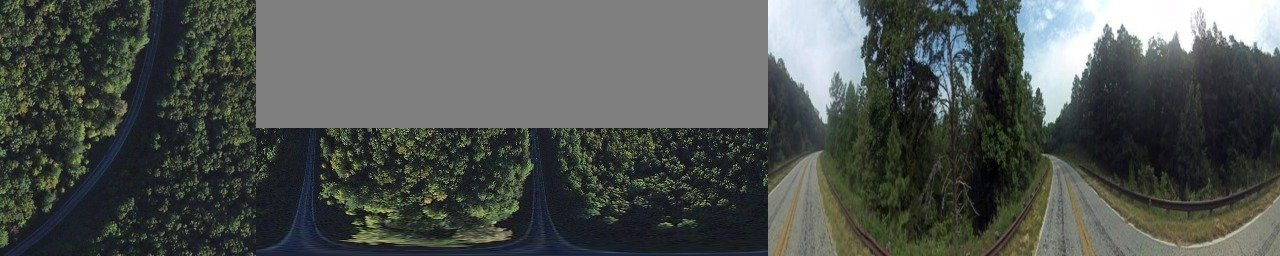
\includegraphics[width=0.8\linewidth]{app_warp_1269.jpg}\\[2pt]
  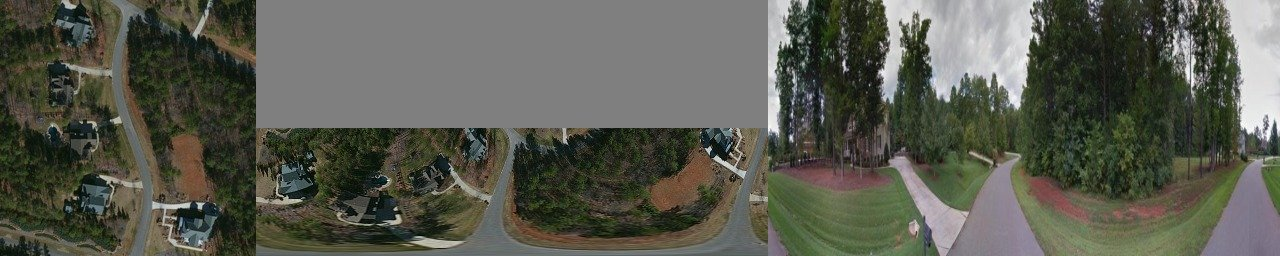
\includegraphics[width=0.8\linewidth]{app_warp_3807.jpg}
  \caption{Warped-aerial check for test images 1269 and 3807, from the warp verification output of the
  released code: the aerial tile, the warped aerial panorama and the real panorama for visual alignment.}
  \label{fig:app_warp}
\end{figure}

% ==================================================================================================
\clearpage
\begin{thebibliography}{99}
\small

\bibitem{zhai2017crossnet}
M.~Zhai, Z.~Bessinger, S.~Workman, and N.~Jacobs.
\newblock Predicting Ground-Level Scene Layout from Aerial Imagery.
\newblock In \emph{CVPR}, 2017. \href{https://arxiv.org/abs/1612.02709}{arXiv:1612.02709}.

\bibitem{workman2015cvusa}
S.~Workman, R.~Souvenir, and N.~Jacobs.
\newblock Wide-Area Image Geolocalization with Aerial Reference Imagery.
\newblock In \emph{ICCV}, 2015. \href{https://arxiv.org/abs/1510.03743}{arXiv:1510.03743}.

\bibitem{regmi2018crossview}
K.~Regmi and A.~Borji.
\newblock Cross-View Image Synthesis using Conditional GANs.
\newblock In \emph{CVPR}, 2018. \href{https://arxiv.org/abs/1803.03396}{arXiv:1803.03396}.

\bibitem{tang2019selectiongan}
H.~Tang, D.~Xu, N.~Sebe, Y.~Wang, J.~J.~Corso, and Y.~Yan.
\newblock Multi-Channel Attention Selection GAN with Cascaded Semantic Guidance for Cross-View Image Translation.
\newblock In \emph{CVPR}, 2019. \href{https://arxiv.org/abs/1904.06807}{arXiv:1904.06807}.

\bibitem{toker2021cdte}
A.~Toker, Q.~Zhou, M.~Maximov, and L.~Leal-Taix{\'e}.
\newblock Coming Down to Earth: Satellite-to-Street View Synthesis for Geo-Localization.
\newblock In \emph{CVPR}, 2021. \href{https://arxiv.org/abs/2103.06818}{arXiv:2103.06818}.

\bibitem{shi2022s2sp}
Y.~Shi, D.~Campbell, X.~Yu, and H.~Li.
\newblock Geometry-Guided Street-View Panorama Synthesis from Satellite Imagery.
\newblock \emph{IEEE Transactions on Pattern Analysis and Machine Intelligence}, 2022. \href{https://arxiv.org/abs/2103.01623}{arXiv:2103.01623}.

\bibitem{qian2023sat2density}
M.~Qian, J.~Xiong, G.-S.~Xia, and N.~Xue.
\newblock Sat2Density: Faithful Density Learning from Satellite-Ground Image Pairs.
\newblock In \emph{ICCV}, 2023. \href{https://arxiv.org/abs/2303.14672}{arXiv:2303.14672}.

\bibitem{li2024crossviewdiff}
W.~Li, J.~He, J.~Ye, et~al.
\newblock CrossViewDiff: A Cross-View Diffusion Model for Satellite-to-Street View Synthesis.
\newblock arXiv preprint, 2024. \href{https://arxiv.org/abs/2408.14765}{arXiv:2408.14765}.

\bibitem{qian2025sat2density}
M.~Qian, B.~Tan, Q.~Wang, et~al.
\newblock Seeing through Satellite Images at Street Views.
\newblock arXiv preprint, 2025. \href{https://arxiv.org/abs/2505.17001}{arXiv:2505.17001}.

\bibitem{isola2017pix2pix}
P.~Isola, J.-Y.~Zhu, T.~Zhou, and A.~A.~Efros.
\newblock Image-to-Image Translation with Conditional Adversarial Networks.
\newblock In \emph{CVPR}, 2017. \href{https://arxiv.org/abs/1611.07004}{arXiv:1611.07004}.

\bibitem{park2019spade}
T.~Park, M.-Y.~Liu, T.-C.~Wang, and J.-Y.~Zhu.
\newblock Semantic Image Synthesis with Spatially-Adaptive Normalization.
\newblock In \emph{CVPR}, 2019. \href{https://arxiv.org/abs/1903.07291}{arXiv:1903.07291}.

\bibitem{oquab2023dinov2}
M.~Oquab, T.~Darcet, T.~Moutakanni, et~al.
\newblock DINOv2: Learning Robust Visual Features without Supervision.
\newblock arXiv preprint, 2023. \href{https://arxiv.org/abs/2304.07193}{arXiv:2304.07193}.

\bibitem{darcet2023registers}
T.~Darcet, M.~Oquab, J.~Mairal, and P.~Bojanowski.
\newblock Vision Transformers Need Registers.
\newblock arXiv preprint, 2023. \href{https://arxiv.org/abs/2309.16588}{arXiv:2309.16588}.

\bibitem{xie2021segformer}
E.~Xie, W.~Wang, Z.~Yu, A.~Anandkumar, J.~M.~Alvarez, and P.~Luo.
\newblock SegFormer: Simple and Efficient Design for Semantic Segmentation with Transformers.
\newblock In \emph{NeurIPS}, 2021. \href{https://arxiv.org/abs/2105.15203}{arXiv:2105.15203}.

\bibitem{zhang2018lpips}
R.~Zhang, P.~Isola, A.~A.~Efros, E.~Shechtman, and O.~Wang.
\newblock The Unreasonable Effectiveness of Deep Features as a Perceptual Metric.
\newblock In \emph{CVPR}, 2018. \href{https://arxiv.org/abs/1801.03924}{arXiv:1801.03924}.

\bibitem{heusel2017fid}
M.~Heusel, H.~Ramsauer, T.~Unterthiner, B.~Nessler, and S.~Hochreiter.
\newblock GANs Trained by a Two Time-Scale Update Rule Converge to a Local Nash Equilibrium.
\newblock In \emph{NeurIPS}, 2017. \href{https://arxiv.org/abs/1706.08500}{arXiv:1706.08500}.

\bibitem{parmar2022cleanfid}
G.~Parmar, R.~Zhang, and J.-Y.~Zhu.
\newblock On Aliased Resizing and Surprising Subtleties in GAN Evaluation.
\newblock In \emph{CVPR}, 2022. \href{https://arxiv.org/abs/2104.11222}{arXiv:2104.11222}.

\bibitem{binkowski2018kid}
M.~Bi{\'n}kowski, D.~J.~Sutherland, M.~Arbel, and A.~Gretton.
\newblock Demystifying MMD GANs.
\newblock In \emph{ICLR}, 2018. \href{https://arxiv.org/abs/1801.01401}{arXiv:1801.01401}.

\bibitem{johnson2016perceptual}
J.~Johnson, A.~Alahi, and L.~Fei-Fei.
\newblock Perceptual Losses for Real-Time Style Transfer and Super-Resolution.
\newblock In \emph{ECCV}, 2016. \href{https://arxiv.org/abs/1603.08155}{arXiv:1603.08155}.

\bibitem{mao2017lsgan}
X.~Mao, Q.~Li, H.~Xie, R.~Y.~K.~Lau, Z.~Wang, and S.~P.~Smolley.
\newblock Least Squares Generative Adversarial Networks.
\newblock In \emph{ICCV}, 2017. \href{https://arxiv.org/abs/1611.04076}{arXiv:1611.04076}.

\bibitem{lin2017focal}
T.-Y.~Lin, P.~Goyal, R.~Girshick, K.~He, and P.~Doll{\'a}r.
\newblock Focal Loss for Dense Object Detection.
\newblock In \emph{ICCV}, 2017. \href{https://arxiv.org/abs/1708.02002}{arXiv:1708.02002}.

\bibitem{zhang2023controlnet}
L.~Zhang, A.~Rao, and M.~Agrawala.
\newblock Adding Conditional Control to Text-to-Image Diffusion Models.
\newblock In \emph{ICCV}, 2023. \href{https://arxiv.org/abs/2302.05543}{arXiv:2302.05543}.

\end{thebibliography}

\end{document}
